\chapter{Background}

\section{What is IoT?}

The Internet Of Things (IoT) is a collective term describing systems of connected computing devices which have the ability to exchange data to other devices. A \emph{Thing} in the internet of things can be a room temperature sensor, a device which tracks geolocation or an actuator which opens or closes a door on command.
\\~\\

\subsection{Relevance of IoT industry}
The IoT space is experiencing an explosive growth, with more than 75 billion devices expected to be connected by 2025 \cite{statista}, nearly a three fold increase from the 2019 figures. In addition, worldwide IoT spending surpassed the 1 Trillion USD figure in 2020 alone \cite{sdx}, with this number expected to increase dramatically in the following years. Consequently, the cost of keeping IoT infrastructure secure has also increased exponentially, with spending on IoT endpoint security solutions reaching 631 million USD in 2021 \cite{gartner}.
\\

\subsection{Critical IoT applications}
IoT applications are numerous and varied. Some IoT applications present no serious danger if malfunctioning or maliciously altered, take for example an IoT system which controls the air conditioning temperature of a room. However, other IoT systems do perform critical tasks, therefore it is important to understand that, if these applications are not performing correctly, either by a design flaw or a malicious attack, these errors can have devastating consequences.
\\

One example of such an attack could be the 2010 Stuxnet virus, which destroyed over 1000 centrifuges used for nuclear-grade uranium enrichment, a similar attack could target IoT systems in charge of monitoring critical task in nuclear facilities. Another example of a critical exploit was discovered when in 2017 attackers exposed a vulnerability in the software of 465.000 pacemakers, making it possible to drain the pacemaker battery, steal sensitive data or even change lifesaving settings on the pacemaker itself.
\\

Many other attacks or system failures are theoretically possible on IoT systems in industries such as healthcare, energy or transportation, to name a few. These systems require some mechanism that can enable them to detect either a system malfunction or an external malicious attack in order to help prevent major damage.


\subsection{Keyloggers}
A keylogger is an application that monitors user inputs in order to gain access to user patterns or private information about the user. 
The American National Institute for Standard and Technology defines a keylogger as \textit{"A remote program designed to record which keys are pressed on a computer keyboard used to obtain passwords or encryption keys and thus bypass other security measures".} Keyloggers are deployed remotely by an attacker to steal information like bank accounts or log in credentials. 

Turning the situation around it should be possible to use a preinstalled application with the same working principle as a keylogger to monitor and detect potential attacks on a device. 

\section{Networking and topologies}

\subsection{What is a network topology}
A network topology is a description of how a network can be organized \cite{network_topologies}. It shows connectivity in the form of nodes and edges in the form of graphs. We have the physical topology that specifically states the type of devices and where they are placed. The logical topology represents the flow of data through the network.

\subsection{Why do we cluster IoT devices?}
Most IoT applications monitor the surrounding environment or acquire data from different devices. To be able to collect and interpret the data in the context of an application we often collect different devices into clusters - a network of IoT devices working together. \\

We can cluster a network of devices based on different criteria like communication range, type of device, purpose of device, localization or transmission power\cite{intrusion_detection}. This is done to provide maximal connectivity through minimum communication to reduce energy usage and computational complexity. A cluster can be composed of several smaller non-overlapping clusters or one large where all devices are connected together.

\subsection{Different types of topologies}
We can adapt several different type of network topologies depending on the usage requirements of the network and characteristics of the connected devices. \\

\subsubsection{Star}
 The star topology is a centralised topology where all nodes are connected to one central node \cite{computer_networking}, figured in the middle of Figure \ref{fig:network_topologies}. This is usually the master node, and has elevated rights. It is also called a server-client structure. If the network is connected to an external point like a cloud or another network segment, it is through the central node. Examples of technologies using star topology is WiFi or wired Ethernet.  

\subsubsection{Mesh}
In a mesh topology, rightmost in Figure \ref{fig:network_topologies}, all devices are connected to each other \cite{computer_networking}. This is a decentralised topology. All devices know the same things and have the same permissions. This provides the possibility of self-scaling networks because nodes functions as relays. This means low-range technologies can reach further than they normally would. Examples of technologies who use a mesh topology are Zigbee and Z-Wave.\\

A mesh topology can be both full and part mesh. In a full mesh all nodes function as relays, while in part mesh only a dedicated set of nodes has this privilege. 

\subsubsection{Point-to-Point}
An established connection between two nodes only \cite{oreilly:IoT_topology}, leftmost in Figure \ref{fig:network_topologies}. It is a low cost solution that is easy to set up and maintain. The main limitation is the restriction in the scalability which is none exceeding the two nodes. This also limits the transmission range of the network to the device with the shortest range. An example of a technology using point-to-point connections is Bluetooth.\\

\begin{figure}[h]
    \centering
    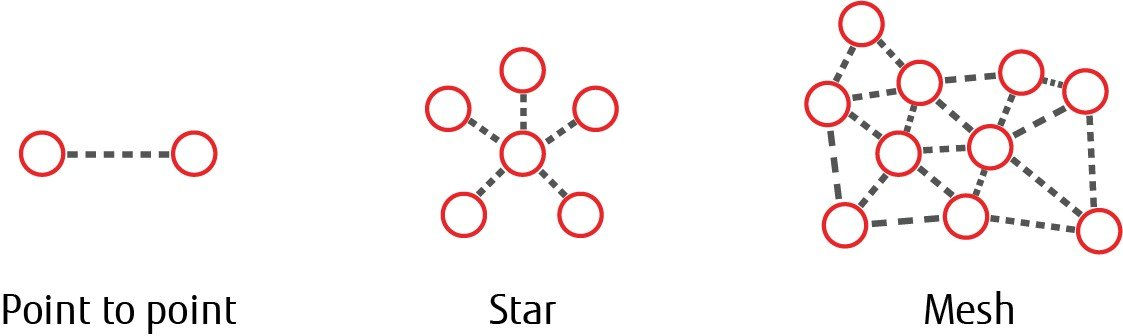
\includegraphics[width=.9\linewidth]{images/network_topologies.jpg}
    \caption{Common IoT network topologies}
    \label{fig:network_topologies}
\end{figure}
  
\subsection{Topologies used in IoT clusters}

All of these topologies can again be organised as flat or segmented. In a flat network all the organizations devices are connected onto the same network. In a segmented one the network is separated into different segments connected by e.g. a router. The segmented solution is preferred from a security aspect as any attack predominantly will be limited to the specific segment. This does on the other hand restrict the agility and feeling of seamlessness within the network.\\

The three topologies mentioned in the previous section are the ones most used in IoT clustering \cite{oreilly:IoT_topology}\cite{linklabs:IoT_topology}. As this project concerns clusters and point-to-point is exclusively between two devices it is natural to take a closer look into the mesh and star topologies.\\ 

Mesh topologies are good for extending networks using short-range protocols like Zigbee and Z-Wave. It is also good if you need bandwidth enough for large data streams. Full mesh is relatively expensive to install, but very fault tolerant in the way all nodes have redundant paths of communication. It allows a high number of nodes in the network, but maintaining all is costly in the form of power consumption. Since a mesh network does not have static routing the timing and latency of the network can vary, making it unfit for time critical applications.\\

From a security aspect mesh topologies are more vulnerable if breached. The moment one relay is breached, all others can be accessed. This vulnerability can be reduced by implementing a part meshed network where only nodes that needs to function as relays will have this privileges. This way e.g. devices like sensors can be attached as leaf nodes. \\

Peter and Perttunen \cite{network_topologies} state that this type of network is most used in military, tactical and other critical applications. This is because of the high degree of reliability, but is also makes the networks more vulnerable, which in turn is more demanding for the remaining security solutions. The consequence of choosing a less ideal network topology is that the remaining security systems potentially need to handle a heavier load. \\

The star topology saves costs where the mesh does not. On the other hand it does not have then same capabilities when it comes to extending the rage of a network since all leaf nodes must be connected to the centre. It is consistent, predictable and fast\cite{oreilly:IoT_topology}.

This makes the star topology an ideal choice if you have a lot of low-level devices like sensors distributed over a confined area. The major drawback of the star topology is that it is reliant on one single gateway. If one of the leaf nodes are attacked the breach is contained within this individual link. If the gateway is breached, an attacker would have full access to the entire network. \\

Topology control is a widely used concept in Wireless Sensor Networks \cite{intrusion_detection}. It is a collection of methods and guidelines on how to cluster IoT applications in a secure way while maintaining integrity, authenticity and reliability. The concept of topology control also mentions network redundancy, which means that it can be useful to deploy a larger number of nodes than what is needed. An increase in nodes increases the attack surface and in turn the vulnerability of the system if the topology control scheme fails.

\subsubsection{Network security threats}
Several scientific articles \cite{electronics:topology_control}\cite{minas_gerais:topology}\cite{intrusion_detection}\cite{IJCSIS:attack_survey} discussing network-topology and control mentions possible attacks related to the networking aspect of an IoT cluster. 

The different attacks has been classified into two groups; one for attacks related to connection to or editing of the nodes composing the cluster. The second for attacks related to normal operations conducted by the network. In Figure \ref{fig:WSN_attacks} below researchers G. Padmavathi and D. Shanmugapriya \cite{IJCSIS:attack_survey} have created a map of possible attacks launched towards Wireless Sensor Networks. As IoT clusters usually contain one or more wireless sensor this is also relevant to this study and several of the attacks will be revisited in the following sections. 

\begin{figure}[h]
    \centering
    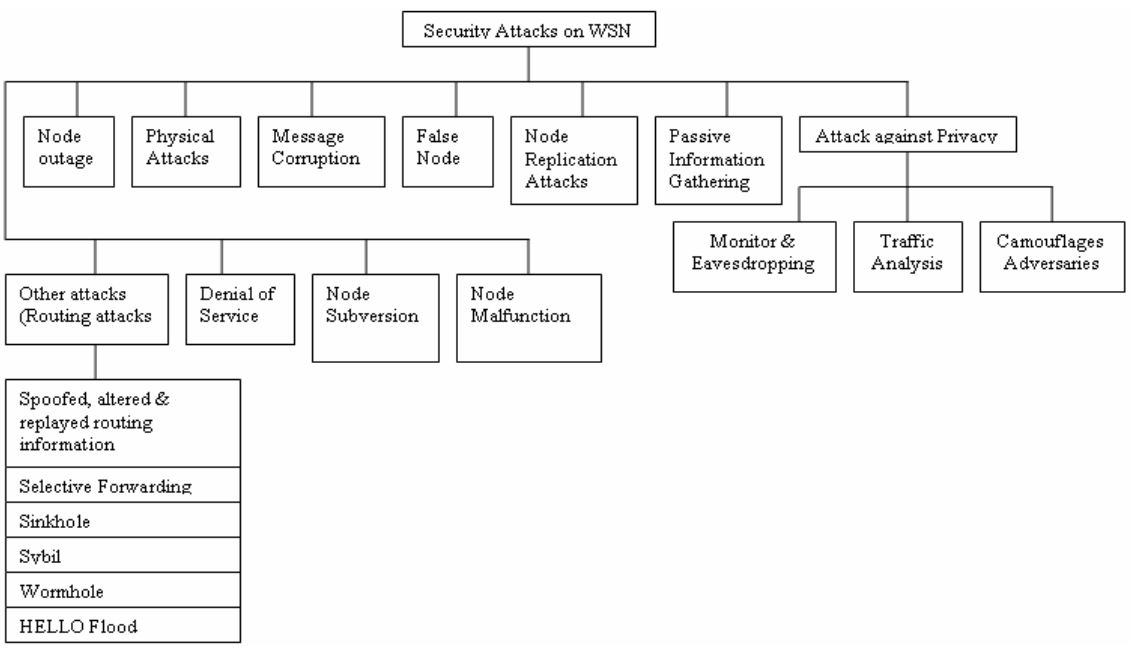
\includegraphics[width=.9\linewidth]{images/attack_classification_WSN.JPG}
    \caption{Classification of possible attacks on WSN \cite{IJCSIS:attack_survey}}
    \label{fig:WSN_attacks}
\end{figure}

\paragraph{Scalability and connectivity} \label{sec:scalability}
An agile network should have the possibility to scale according to user needs. This means adding or removing nodes without necessarily reconfiguring the entire network.

Nodes in different places of the network topology uses different amounts of energy. If a node is used for relay purposes it will use more energy. Because of this the energy signature of a node can be used to decide which nodes should be breached \cite{electronics:topology_control}. Unfortunately it is not possible to monitor if a attacker is monitoring the signature without extra sensors or equipment.

\paragraph{Node subversion} \label{chap:node_tampering}
The attacker steals or tampers with an already existing node in order to steal information or modify transmissions in and out of the node. As the existing node is already connected to the network the cryptographic keys become vulnerable.

\paragraph{False nodes}
An attacker adds a false node to the system in order to obtain information about the network or interrupt transmissions between real nodes. A false node can also be used to conduct a network flooding attack which is similar to a DoS attack where the false node overloads network capacity by flooding the network with useless information. A false node can also be used to conduct a MitM attack. 

\paragraph{Node Replication}
Similar to a false node attack. The attacker replicates the ID of an existing node and impersonates this node to flood the network or inject false information. 

\paragraph{Node outage}
Old or outdated nodes are not an attack in itself but can in worst case be exploited by an attacker to gain access to the rest of the functional network. It can also lead to the node malfunctioning and expose the integrity of the network. 

\paragraph{Routing attacks}
All networks require information to be routed around according to some routing philosophy. The routers in charge of forwarding packets can be attacked in a number of ways \cite{IJCSIS:attack_survey}. 

\begin{itemize}
    \item Spoofed or altered
    \item Selective forwarding
    \item Sinkhole attack
    \item Sybil Attacks
    \item Wormhole attacks
    \item HELLO flood attacks
\end{itemize}

All of these attacks have in common that they affect the network layer and the behaviour of the router is altered to either dismiss or snatch up messages.

\subsubsection{General network attacks}
The following attacks can happen to or between any node. The attacks can be more or less likely depending on the type of protocol used to implement the network topology. 

\paragraph{Eavesdropping}
Snapping up amounts of data traffic to discover the content of messages sent on the network. Also known as sniffing or snooping. 

\paragraph{Traffic analysis}
Analyzing the traffic sent over the network to deduct patterns of usage or other information even if the information is encrypted. 

\paragraph{Denial of Service} 
In a DoS attack the attacker exhausts the networks resources by sending spam data and thus prevents real nodes from sending their data. DoS attacks can again be divided into authentication request flooding, Association request flooding, Rouge Spoofing, CTS/RTS and injection of malicious packets \cite{intrusion_detection}. A DoS attack can lead to network failure which in turn leads to a disconnected system. Jamming is a type of DoS attack which prevents nodes from communicating by completely occupying a channel or port. 


\paragraph{Normal operation states}
As discussed in Section \ref{sec:scalability}, changes in network topology are normal operations. At the same time many attacks are also connected to these types of activities. This makes it natural to monitor operations like addition, removal and reconnection of nodes. 

There is also a rage of attacks targeting routers. In these attacks the routing stream of packages is altered from the natural created by a routing algorithm. If a routing algorithm works correctly it should distribute traffic evenly or at least avoid any router from exceeding bandwidth capacity. In this case the load on each router should be monitored and compared.

 
\paragraph{Attack signatures}
Some attacks uses methods that are easily recongnized and can be classified as attack signatures. The group of attacks included in Denial of Service all have in common that a large increase in packets or requests are injected into the network. For this type of attacks it could be useful to monitor all occurrences where a high frequency of packets or requests are detected on the input port of a node.  \\

A Man in the Middle attack is more difficult to detect but a normal approach is to monitor changes in RTT of packets sent between nodes, as this is likely to increase during a MitM attack. This is on the other hand pointless if the implemented topology is mesh where routing is dynamic. The strength of the transmission signal is also likely to decrease since an attack often is conducted further away than the location of the device. This again only works when the distance between the communicating nodes is fixed. \\

To avoid an attacker from exploiting outaged nodes production date or performance indices of nodes should be monitored to ensure they do not exceed some threshold. This is not specifically an attack signature, but it is a signature that can be used as a preventive asset. 













\section{IoT communication protocols}

IoT devices come in all shapes and sizes and used in a wide range of applications, but they share one common main goal, to collect and transmit data. Communication can either be wired or wireless, where the main concern for this kind of smart devices is the latter. Since there is no unique standard, multiple communication protocols are in use, depending on the requirements, such as, the data bandwidth, the radio range, the power consumption, the  topology or the security constraints. \\

This section will describe the main protocols used in IoT communications, as well as the advantages and disadvantages between them. Typically, the type of connectivity is given by the distance the data must travel, in such scenario, it is possible to divide the most common network protocols in two categories: \textit{Low-power, wide-area networks (LPWAN)} and \textit{Low-power, short-range networks} \cite{Microsoft:protocols}. The classification diagram is shown in figure \ref{fig:NetworkClassification}.


\begin{figure}[h]
    \centering
    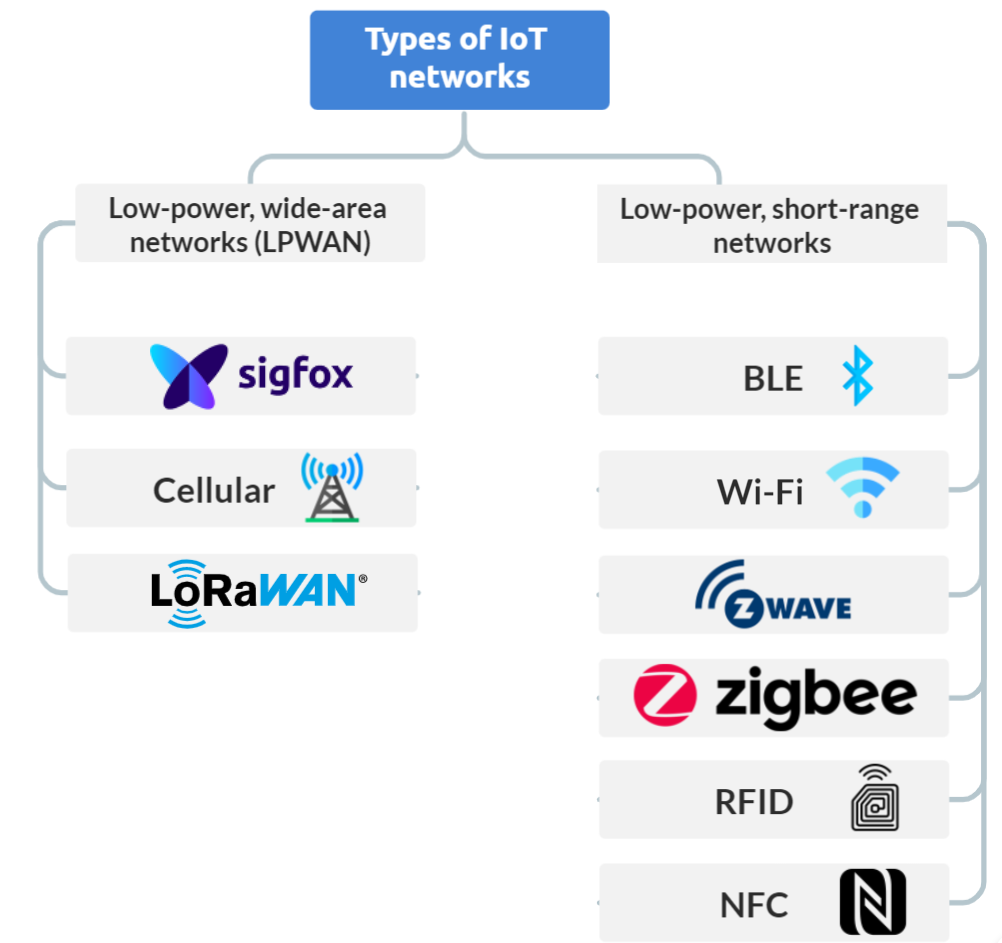
\includegraphics[width=.9\linewidth]{images/TypeOfNetworks.png}
    \caption{IoT network classification}
    \label{fig:NetworkClassification}
\end{figure}


\subsection{Low-power, wide-area networks (LPWAN)}
The main characteristic of LPWANs is to provide long-range communication on low-power devices. These protocols are better suited for applications that do not require high bandwidth or time-sensitive constraints \cite{BehrTech:protocols}.

\subsubsection{Sigfox}
The Sigfox technology is intended for Machine-to-Machine (M2M) communication. It uses an Ultra Narrow Band channel, making data transfer speed as low as 10 to 1000 bps. On the other hand, distance between nodes can go up to 50 Km \cite{IEEE:protocols}.

\subsubsection{Cellular}
Although cellular networks are under the LPWAN category, they are not by any means cheap on power, on the contrary they impose high power requirements, but provide high speed communication over long distances, taking advantage of the installed GSM/3G/4G/5G mobile networks. Cellular technology is not viable for most IoT devices, since they are battery-operated.

\subsubsection{LoRaWAN}
The Long-Range Wide-Area Networks (LoRaWAN) is intended for transmitting small size payloads over long distances. Devices supporting this technology are optimized to operate in a low power mode, lasting up to 10 years on a single cell battery. Signals can be sent and received over a distance of 3 km in urban areas or 10 km in rural areas. The network is secured by end-to-end AES-128 encryption \cite{LoRaWAN}.

\subsection{Low-power, short-range networks}
This type of networks are better suited for homes, offices or small environments, since they can support short range communication, with the advantage of being inexpensive to operate and require small batteries.

\subsubsection{Bluetooth Low Energy (BLE)}
BLE is very significant protocol in the IoT world. According to the 2022 market report written by Bluetooth \textregistered, It is estimated that about 35\% of all IoT connected devices rely on this protocol \cite{BLE1}.
BLE was designed for short-range communications with low latency, but with low bandwidth. However it takes into account a very low power consumption. We can find devices relying on this technology in audio streaming devices, PC peripherals, accessories and fitness and health wearables. Nowadays, also very common in asset tracking and indoor navigation where GPS can not be used.

\subsubsection{Wi-Fi} \label{sec:wifi}
Wi-Fi technology is pretty much spread all over, including IoT applications. It provides high-throughput data transfers. However, due to its high imposing energy requirements, WiFi is not a feasible network protocol for IoT running on batteries. Instead, it is more suitable for devices that are connected to the power outlet, as security cameras or smart home appliances. The allowed distance is usually within the range of 35 m indoors and 100 m outdoors \cite{IEEE:protocols2}.

\subsubsection{Z-Wave}
It is a standard designed for remotely controlled residential applications, it can deliver a transmission speed of 40 kbps reaching up to 30 m. It uses AES-128 encryption for securing the channel \cite{IEEE:protocols2}.

\subsubsection{Zigbee}
This protocol is based on the IEEE 802.15.4 standard, it is intended for short-range low-power communications, typically deployed in mesh topologies to extend the coverage. It provides a low bit rate up to 250 kbps. It is possible to connect 65000 nodes in a single zigbee network. Operates in a rage of 10 to 100 meters 

\subsubsection{RFID}
Radio Frequency Identification (RFID) consists of small readers and RF tags transmitting small amount of data through radio waves within very short distances. RF tag are electronically programmed with unique information, so they cannot be used to collect measurements. However, RFID has had a great positive impact in retail and logistics, as tags can be attached to all kind of products for inventory tracking.

\subsubsection{NFC}
Near-Field Communication (NFC) is a protocol very similar to RFID. It can connect two devices in a distance shorter than 4 cm. It can be used for identification (similar to RFID), but also for more capable two-way communication. This technology is now extended to mobile phones, contactless payments and different industrial applications.\\

Table \ref{tab:DiffNetworks} provides a comparison between the different network protocols most used in IoT scenarios \cite{IEEE:protocols}.

\begin{table}[]
\centering
    \resizebox{\textwidth}{!}{\begin{tabular}{lcccc} 
         \hline
         Technology & Range & Data Rate & \makecell{Power \\consumption} & Topology \\ 
         \hline
         Sigfox & \makecell{10 km (urban) \\ 50 km (rural)} & \makecell{100 bps (urban) \\ 600 bps (rural)} & 10 - 100 mW & Star \\ 
         Cellular & Several km & 8Mbps (3G), 50Mbps (4G) & High & -\\ 
         LoRaWAN & 	$<$ 10 km & 27 kbps & High & Start\\
         \hline
         BLE & 15 - 30 m& 1 Mbps & Low (30 mA) & Star-bus\\
         Wi-Fi & $<$ 100 m & $>$ 100 Mbps & High & Start, Mesh \\
         Z-Wave & $<$ 30 m & 40 kbps & Low (2.5 mA) & Mesh \\
         Zigbee & 10 - 100 m & 250 kbps & Low (30 mA) & Star, Mesh\\
         RFID &  200 m& 4 Mbps& Ultra-low & Point-to-Point\\
         NFC & $<$ 4 cm & 106, 212, 424 kbps& 50 mA& Point-to-Point\\
         \hline
    \end{tabular}}
    \caption{Comparison between network protocols}
    \label{tab:DiffNetworks}
\end{table}













\section{FreeRTOS monitoring} \label{chap:freertos}

This project regards IoT clusters where the devices are running the FreeRTOS operating system. This chapter looks closer into the OS itself and how different attacks can be detected in terms of behavioural changes in the system. \\ 

\subsection{FreeRTOS}

The FreeRTOS is a open source real-time OS created for microcontrollers and small microprocessors \cite{manual:freeRTOS}. It is well suited for systems with both soft and hard real-time requirements. Using the kernel allows the programmer to leave timing to the OS, as well as modularity, easier maintainability and several other benefits.\\

The OS implements a real-time kernel in the shape of a scheduler in order to allow different processes to run independently. The scheduler can also exploit several cores to run concurrent processes. In the FreeRTOS a process is called a thread, but it will be reffered to as a process or a task. To be able to schedule the different threads of the system to the right time the OS use priorities. It is pre-emptive, meaning running processes can be interrupted and suspended to allow a process with higher priority to run. The priorities are configured such that a low numerical value corresponds to a low priority task, with zero being the lowest possible priority.\\

Processes can communicate using semaphores; both binary and counting, queues, mutexes and events. The OS is built up by a library of source and header files. There are two distributions of the OS - one providing the bare minimum of functionality and one supporting amongst other several communication protocols. For this project the basic version of the FreeRTOS was examined and is therefore the one referred to here. To build the kernel different source files need to be configured but the standard project requires files.\\

\begin{itemize}
    \item tasks.c
    \item list.c
    \item queue.c
    \item timers.c
    \item event\_groups.c
    \item croutine.c - only if event groups are used
\end{itemize}
 


\subsection{Monitoring to detect attacks} \label{chap:freertos_monitor}

For a keylogger to be effective it must provide the recipient with useful information. This means that the goal must be to monitor both extraordinary events that are not in the normal behavioural pattern of the application and changes in normal behaviour. \\

An important remark is that to be able to provide such useful information knowledge of the specific system and its user patterns is needed. Simply logging all events might not prove useful but will often be connected with a certain threshold or pattern. This is further explained and examplified in Chapter \ref{chap:real_world_app}.  


\subsubsection{Change in memory usage}
If the rate of memory accesses changes drastically over a specified interval this can be a sign that an attacker tries to fill the devices memory. This could be connected to certain areas in memory storing critical data. The attack signature could match a buffer overflow attack, where the attacker purposely write excessive data to a buffer to gain access to the program memory of the device \cite{buffer_overflow}. This type of attack would be closely connected to the hardware and the hardware abstraction layer of the software rather than the OS itself. 

\subsubsection{Scheduling}
A way of launching a DoS attack on an operating system level could be to request the device to launch a series of high-priority tasks resulting in the system starving lower-priority task even if they are necessary to perform. It could also be as simple as launching too many tasks at once. This could be monitored by logging the number of current existing tasks and the priority of the respective tasks. An alternative to the starvation case could also be to measure the time passed after violating a hard real-time task requirement. 

\subsubsection{Communication}
If a node in the network is attacked, a potential next step for the attacker could be to try disable central nodes by launching a another type of DoS attack where the attacker requests connection or other sorts of data. In that case, the frequency of sockets opened in the node could be monitored and if an attack within the node itself is suspected, one could also note the frequency of tasks filling the socket for sending.\\

For rigid IoT clusters the number of nodes are rarely changed and most devices are online for the most of the time. For these cases monitoring the number of open ports and their belonging IP addresses could help detect node subversion and addition of false nodes. 













\section{IoT Attacks and Safety implications}

\subsection{IoT Vulnerabilities}
Since IoT devices have applications in many different fields, each with varying energy and hardware constraints and with different communication methodologies, the attack surface for cybercriminals is very wide. Design of IoT devices needs to carefully examine the potential vulnerabilities and the corresponding protections that need to be implemented.\\
    
To aid in the detection and prevention of attacks, and the development of security systems to protect IoT devices, multiple security principles have been identified by Staddon, E. et al \cite{IoT_categorization}, shown in Figure \ref{fig:security_principles} below. These need to be addressed in the design phase to achieve a secure design.\\

\begin{figure}[h]
    \centering
    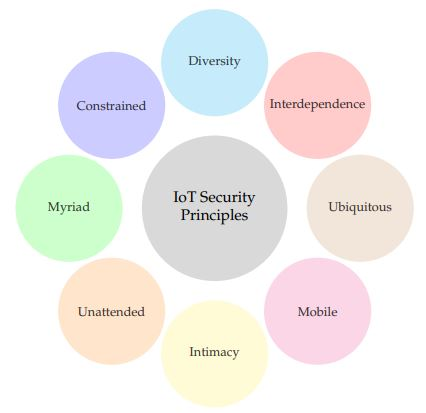
\includegraphics[width=.8\linewidth]{images/IoT security principles.JPG}
    \caption{IoT security principles proposed in the paper}
    \label{fig:security_principles}
\end{figure}

Take for example the Interdependence security principle, it states that since IoT systems are increasingly interconnected, the need for human interaction is diminished and allows for attackers to modify the system's behaviour by interfering with a single device. One real world use case would be a set of smart lightbulbs controlled by a light sensor, if the attackers gained control of the light sensor, they could send some malicious information to turn off the lightbulbs and irrupt into the house undetected.


\subsection{Types of attacks on IoT devices}
The same report by Staddon, E. et al \cite{IoT_categorization} proposes several categorization methods for IoT attacks, including labeling attacks based on the severity of the attack, the attack type or the access type, to name a few.\\

One of the proposals is to divide the attacks into three level related categories, \emph{Low-level}, \emph{Intermediate-level} and \emph{High-level} security issues. Low-level security issues encompasses threats to the lowest network layers, but also to the device's physical state. This includes attacks such as jamming, which disrupts network communication by saturating the communication channel or Denial of Sleep, in which the IoT device is constantly "kept awake" by issuing requests or by other means and this way the battery of the device is drained considerably more rapidly than it normally would. A DoS attack, another type of low-level attack is ARP-Spoofing, where a malicious attacker can access, modify or even stop data-in transit by obtaining a legitimate computer's IP address through malicious Address Resolution Protocol (ARP) messages.\\

Intermediate-level attacks are labeled as those directed against the network and all transport layer related activities, such as a routing and session management. Some examples of Intermediate-level attacks are Replay attacks, where data transmission is maliciously repeated or delayed, or a Sinkhole attack, where a malicious set of nodes modify the network traffic in order to prevent the base node from receiving the correct information.\\

The final High-level attacks are those that target the application itself, they revolve around application vulnerabilities, such as insecure public interfaces, causing a breach to data privacy, or insecure software/firmware, allowing the attacker to take advantage of injection attacks like SQL or XML-injection.\\

It is important to highlight that this is just one of the dozens of categorization methods that exist for cyberattacks on IoT devices. From a security perspective it is interesting to study several categorization methods and offer protection against the types of attacks a specific IoT system might be vulnerable to.\\


\subsection{Safety and security implications of IoT attacks}
Since the attack surface on IoT devices is so big, many different severe consequences can result from a successful IoT cyberattack, we will look at some real world examples to understand the scale of the damage that could be inflicted.
\\~\\
One example would be the exploit of a \hyperlink{https://thehealthcareblog.com/blog/2019/07/29/security-crisis-of-cardiac-pacemakers-paves-the-way-for-iot-security-evolution-in-cardiology/}{vulnerability detected in 475k pacemakers}, this attack would expose critical health parameters of thousands of people that could be manipulated to cause harm/death.
\\~\\
Another IoT system in which attacks could have critical consequences is the smart-cars, which are rising in popularity, and \hyperlink{https://www.lifewire.com/how-self-driving-cars-can-be-hacked-5114337}{many possible attacks have already been proven to exist}, endangering not only the occupants of the car, but also other external actors. 
\\~\\
In general, we can observe that the IoT industry is vulnerable to many different types of attacks with very high damage potential, which is why protection, prevention and detection of these attacks is extremely necessary.


